\documentclass[10pt, aspectratio=169]{beamer}
\usepackage{caption}
\usepackage{subcaption}
\usetheme[progressbar=frametitle]{metropolis}
\usepackage{amsmath}
\usepackage{siunitx}
\usepackage{xcolor}
%\usecolortheme{crane}
\definecolor{craneorange}{rgb}{0.53,0.66,0.42}
\usecolortheme{spruce}
\usepackage{hyperref}
\usepackage{multimedia}
\usepackage[percent]{overpic}
%\usepackage[para]{footmisc}

%\title{Parallel High-order Multi-component compressible flows on unstructured mesh}
\title{Computational study of acoustic waves emitted by collapsing bubbles}
%\subtitle{Ph.D. monitoring meeting}
\date{\today}
\author[shortname]{Magu Raam Prasaad R}
%\author[shortname]{Dipak Vaghani \inst{1}}
%\institute[shortinst]{\inst{1} Indian Institute of Science}
%\pgfdeclareimage[height=0.5cm]{university-logo}{IIScLogo-High-Res}
%\logo{\pgfuseimage{university-logo}}

\begin{document}
\begin{frame}
	\maketitle
\end{frame}
\begin{frame}
	\frametitle{Motivation - Acoustic waves emitted by collapsing bubbles}
	\begin{columns}
		\column{0.5\textwidth}
		\begin{itemize}
			\item High-speed flows lead to the formation of cavitation bubbles.
			\item Collapsing cavitation bubbles form blast and shock waves.
			\item Blast wave emission process - strong source of acoustic waves.
		\end{itemize}
							
		\column{0.5\textwidth}
		\begin{figure}[h]
			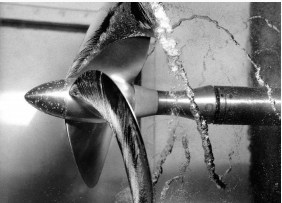
\includegraphics[scale = 0.55]{propeller.png}
			\caption{Cavitation bubbles around rotating propeller\cite{propeller}}	
		\end{figure}
							
	\end{columns}
	\footnotetext[1]{Brennen C. E, JFM 2002}
\end{frame}

\begin{frame}
	\frametitle{Motivation - Acoustic waves emitted by collapsing bubbles}
	\begin{columns}
		\column{0.5\textwidth}
		\begin{itemize}
			\item Emitted acoustic waves interact with the deforming bubbles.
			\item Bubbles strongly interact with and produce sound.
			\item Bubble interaction alters the spectrum of acoustic signal.
		\end{itemize}
							
		\column{0.4\textwidth}
		\movie{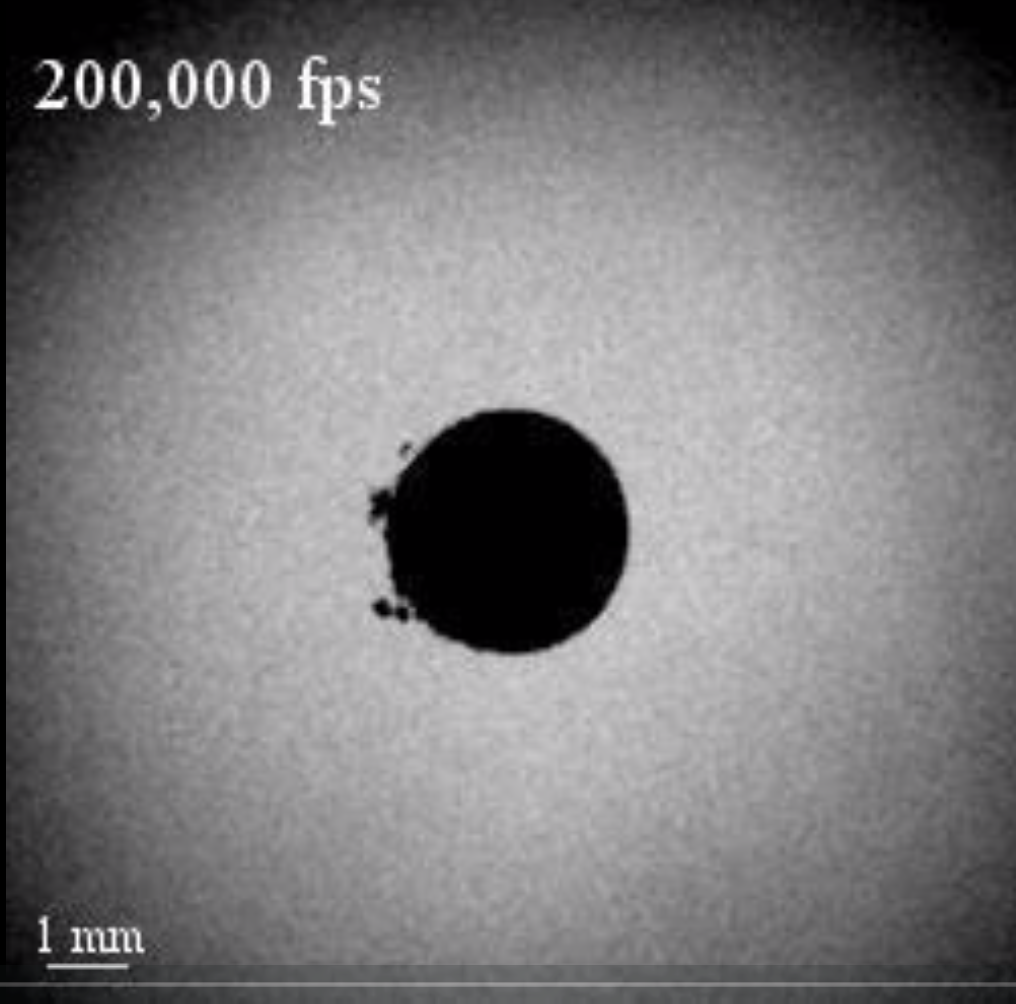
\includegraphics[scale=0.15]{bubble_anima.png}}{bubble_anima.avi}
	\end{columns}
	\footnotetext[2]{Animation source: O. Supponen, PhysRevFluids 2017}
\end{frame}

\begin{frame}{Objective and computational challenges}
	Objective:
	\begin{itemize}
		\item To simulate single and multiple cavitation bubble collapse processes.
		\item To analyse the acoustic wave generation and propogation.
	\end{itemize}
	Computational challenges:
	\begin{itemize}
		\item Bubbles are highly compressible and water is nearly incompressible.
		\item Bubbles occur in clusters.
		\item Collapse process is fast and violent.
		\item Emission of blast and shock waves.
		\item Sound waves can propogate large distances without dissipation.
	\end{itemize}
\end{frame}

\begin{frame}{Computational approach: Flow solver}
	
	High-speed compressible multiphase flow solver developed in the lab.
	\begin{itemize}
		\item with shock and interface capturing\cite{interface}.
		\item low dissipative higher order discretization (WENO-ADER\cite{ADER}).
		\item Massively parallel.
		\item Both structured and unstructured grid.
		\item Using deal-ii\cite{dealii} and PETSc library.
	\end{itemize}
	\footnotetext[5]{Shukla et al. Journal of Computational Physics. 2010}
	\footnotetext[3]{M. Dumbser, J. Sci. Comput. 2017}
	\footnotetext[4]{A General Purpose Object Oriented Finite Element Library}
\end{frame}

\begin{frame}{Bubble collapse near a rigid wall}
							
	\begin{columns}
		\begin{column}{0.45\textwidth}
			\begin{itemize}
				\item air bubble in water
				\item Rectangular domain $\Omega = [-2,5]\times[-5,5]$
				\item Radius of the bubble $R = 10mm$
				\item Discretization $350\times 500$ cells
				\item Boundary conditions:
				      \begin{itemize}
				      	\item left boundary $-$ reflective
				      	\item top, bottom and right boundary $-$ transmissive 
				      \end{itemize}
			\end{itemize}
		\end{column}
																																			
		\begin{column}{0.46\textwidth}
			\begin{figure}
				\centering
				\begin{overpic}[scale=0.25,unit=1mm]{air_bubble_initial.png}
					\put (32,76) {$\displaystyle \textcolor{white}{Water}$}
					\put (32,69) {\textcolor{white}{$\displaystyle \rho = 10^{3}$ $kgm^{-3}$}}
					\put (32,62) {\textcolor{white}{$\displaystyle p = 100.0$ Pa}}
																																							
					\put (15,48) {$\displaystyle \textcolor{white}{Air}$}
					\put (15,35) {\textcolor{white}{$\displaystyle \rho = 0.001 $ $kgm^{-3}$}}
					\put (15,28) {\textcolor{white}{$\displaystyle p = 1.0$ Pa}}
				\end{overpic}
				\caption{Initial condition}
			\end{figure}
		\end{column}
														
	\end{columns}
\end{frame}

\begin{frame}{Bubble collapse near a rigid wall: Density field}
    \centering
	\movie{ 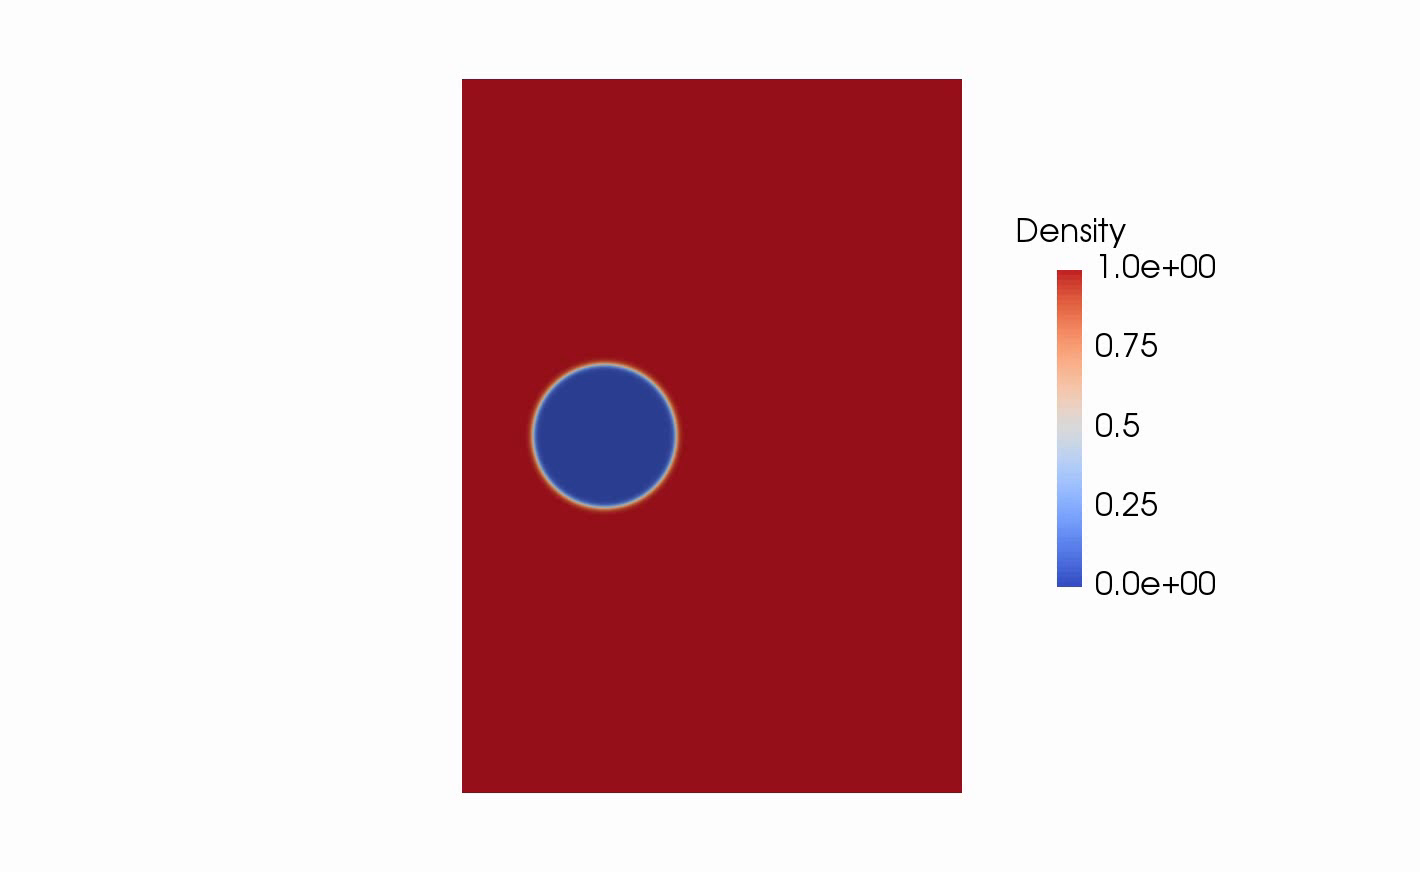
\includegraphics[scale=0.23]{bubble_animation.png} }{bubble_animation.avi}
\end{frame}

\begin{frame}{Bubble collapse near a rigid wall: Numerical schlieren}
    \centering
    \movie{ 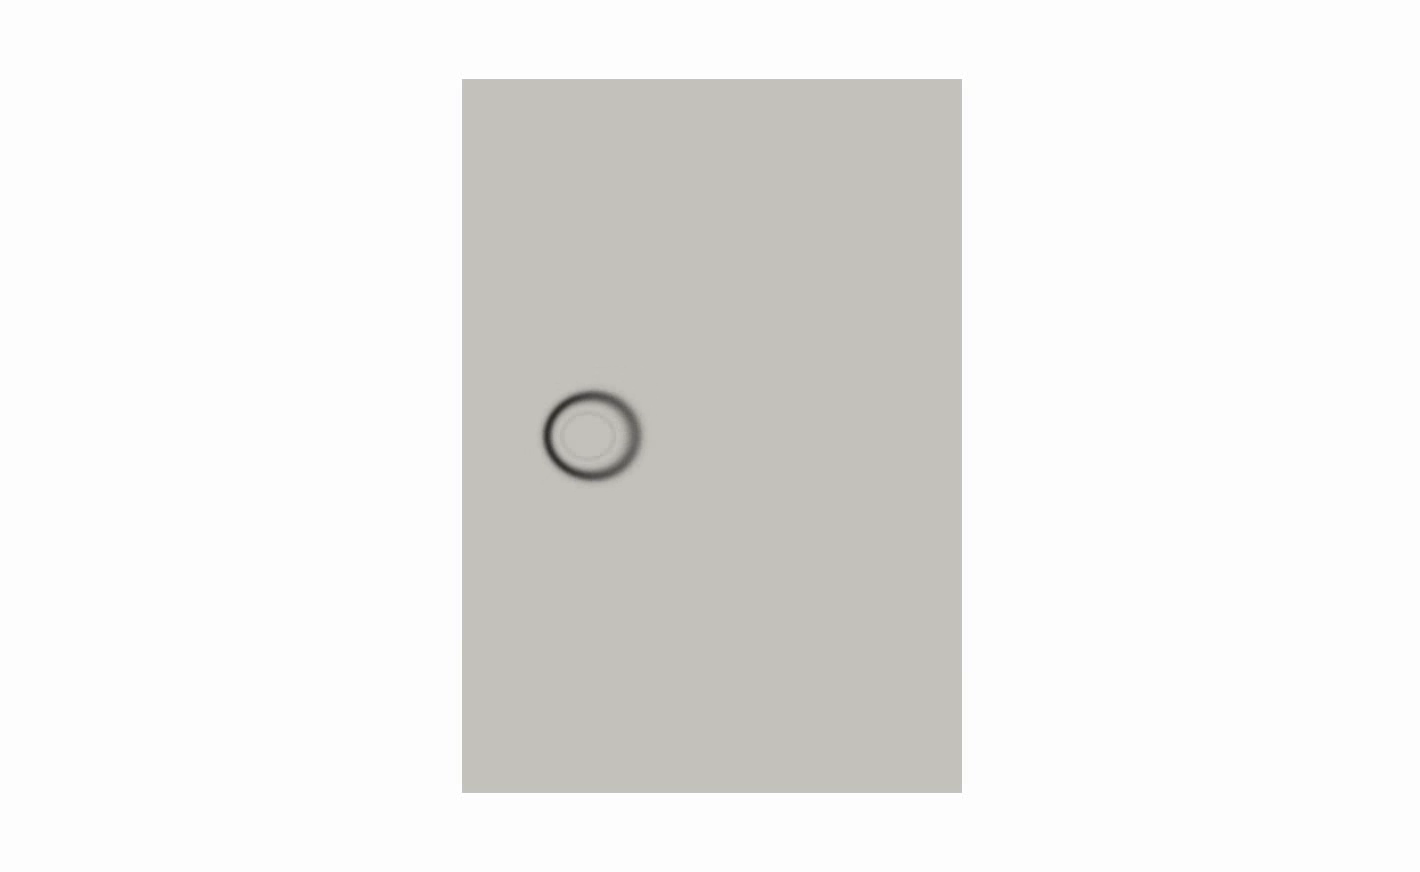
\includegraphics[scale=0.25]{schlieren.png} }{schlieren.avi}
\end{frame}

\begin{frame}{Bubble collapse near a rigid wall: Blast waves}
    \centering
    \movie{ 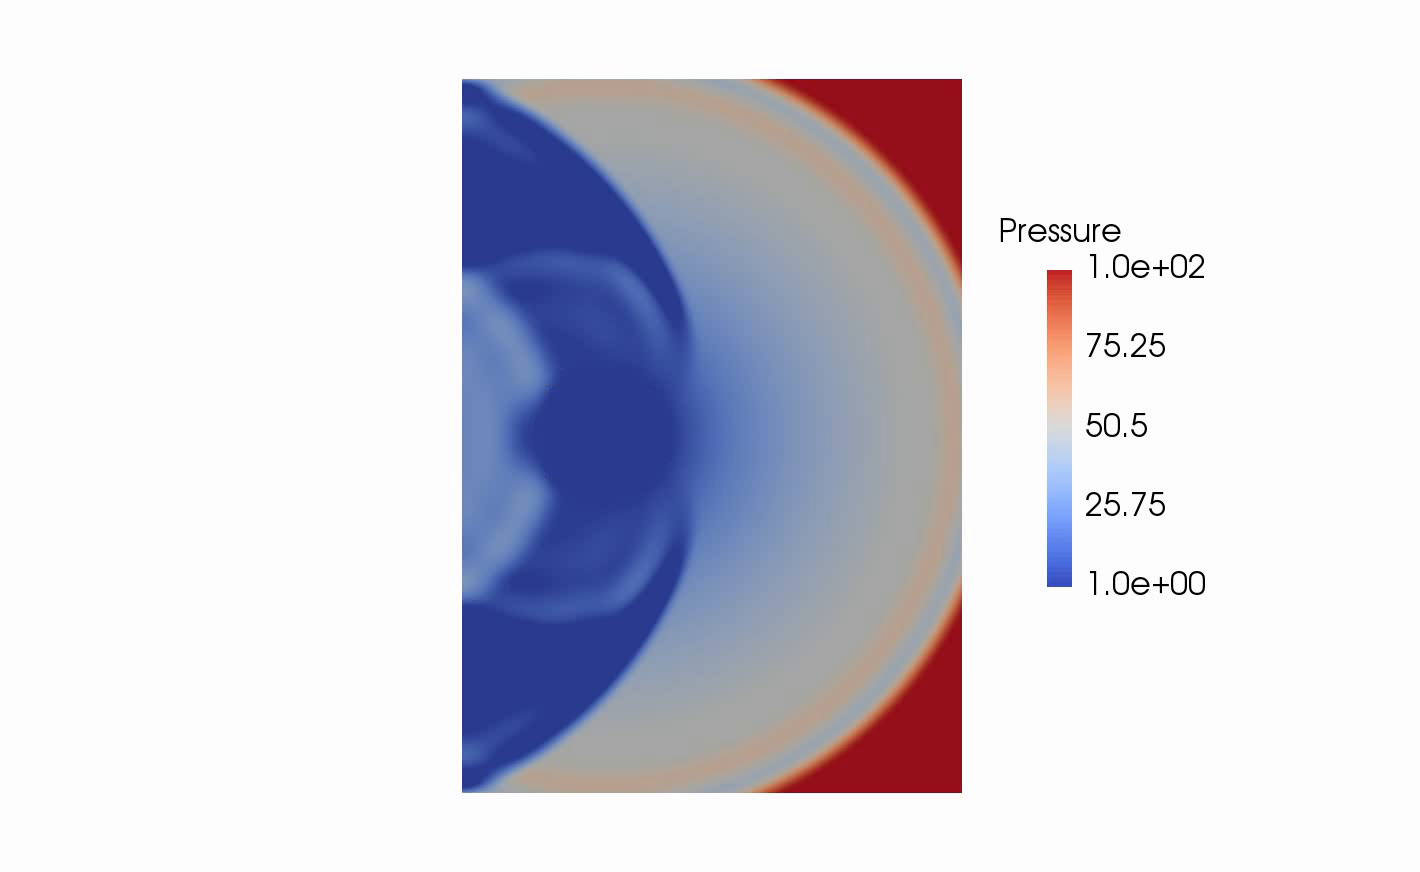
\includegraphics[scale=0.25]{blast_waves.png} }{blast_waves.avi}
\end{frame}


\begin{frame}{Acoustic solver}
	\begin{itemize}
		\item Acoustic wave equation
		\begin{equation}
			\frac{\partial{}^{2}{u}}{\partial{t}^{2}}- c^{2}\nabla{}^{2}{u}=0
		\end{equation} 
		\item Spatial discretization 
		\begin{itemize} 
			\item 2d structured and unstructured grid
			\item finite-volume discretization
			\item 4th order central weno polynomial
		\end{itemize}
		\item Temporal discretization
		\begin{itemize} 
			\item SSPRK54 scheme
		\end{itemize}
	\end{itemize}
\end{frame}

\begin{frame}{Test Case 1: Structured grid - Standing wave solution}
																	
	\begin{columns}
		\begin{column}{0.45\textwidth}
			\begin{itemize}
				\item 2d structured grid $\Omega = [-1,1]\times[-1,1]$
				\item homogeneous Dirichlet boundary condition.
				\item Initial condition:
			\end{itemize}
			$$u(x,y,0) = sin(k_{x}x)sin(k_{y}y)$$
			$$\frac{\partial u(x,y,0)}{\partial t} = 0$$
			where $k_{x} = {2\pi}$, $k_{y} = {2\pi}$, $\omega = \sqrt{8}\pi$
		\end{column}
																																			
		\begin{column}{0.45\textwidth}
			\begin{figure}
				\centering
				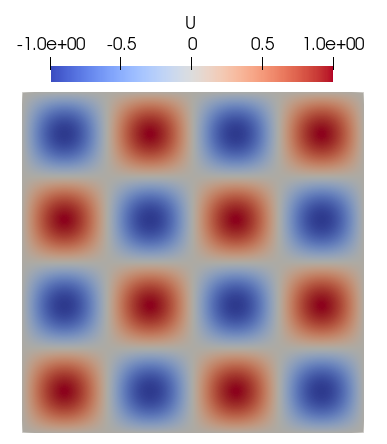
\includegraphics[scale=0.38]{standing_wave.png}
				\caption{standing wave at t = 0.}
			\end{figure}
		\end{column}
	\end{columns}
\end{frame}



\begin{frame}{Rate of Convergence - Standing wave solution}
	\begin{columns}
		\begin{column}{0.45\textwidth}
			\begin{itemize}
				\item 4th order convergence in space
				\item $L_{\infty}$ error is 3.12e-06 after 100 cycles for resolution (N/$\lambda$ = 50)
				\item Low numerical dissipation
			\end{itemize}
		\end{column}
		\begin{column}{0.55\textwidth}
			\begin{tabular}{ |c|c|c|c|c| } 
				\hline
				N   & $L_{\infty}$norm & $L_{2}$ norm & $L_{2} rate$ & $L_{\infty} rate$ \\ 
				\hline
				32  & 1.60e-03         & 8.32e-04     & -            & -                 \\
				64  & 1.06e-04         & 5.35e-05     & 3.95         & 3.91              \\
				128 & 6.73e-06         & 3.37e-06     & 3.98         & 3.97              \\
				256 & 4.22e-07         & 2.11e-07     & 3.99         & 3.99              \\
				\hline
			\end{tabular}

		\end{column}
	\end{columns}	
\end{frame}

\begin{frame}{Test Case 2: Unstructured grid - Plane wave solution}
																	
	\begin{columns}
		\begin{column}{0.45\textwidth}
			\begin{itemize}
				\item 2d unstructured periodic grid
				\item sinusoidal perturbed periodic domain $\Omega_p = [-8,8]\times[-8,8]$
				\item Initial condition:
			\end{itemize}
			$$u(x,y,0) = sin(k_{x}x + k_{y}y)$$
			$$\frac{\partial u(x,y,0)}{\partial t} = -\omega cos(k_{x}x + k_{y}y)$$
			where $k_{x} = {\pi}/{2}$, $k_{y} = {\pi}/{2}$, $\omega = 2\pi$
		\end{column}
																																			
		\begin{column}{0.45\textwidth}
			\begin{figure}
				\centering
				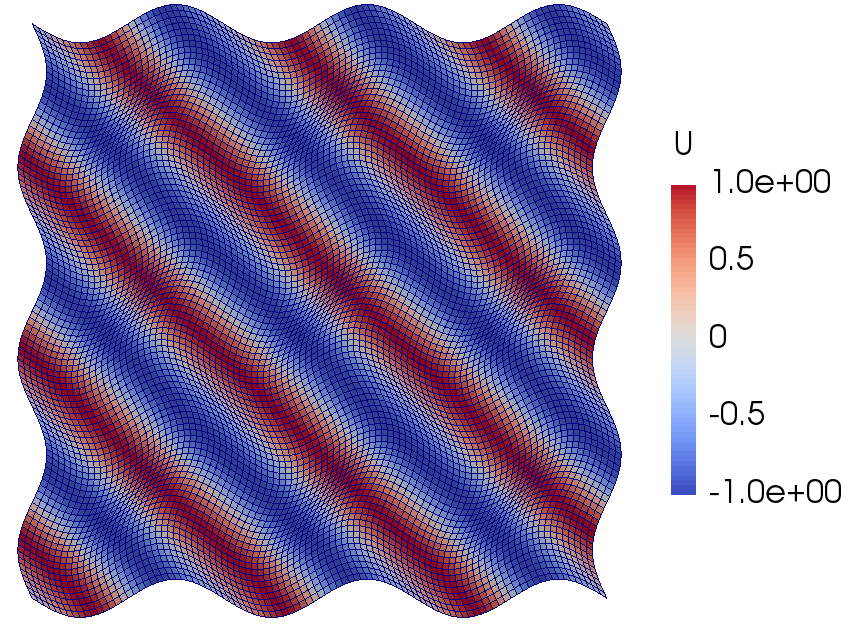
\includegraphics[scale=0.23]{plane_wave_grid.png}
				\caption{plane wave at t = 0.}
			\end{figure}
		\end{column}
	\end{columns}
\end{frame}

\begin{frame}{Rate of Convergence - Plane wave solution}
	\begin{columns}
		\begin{column}{0.45\textwidth}
			\begin{tabular}{ |c|c|c|c|c| } 
				\hline
				N   & $L_{\infty}$norm & $L_{2}$ norm & $L_{2} rate$ & $L_{\infty} rate$ \\ 
				\hline
				32  & 1.12e-03         & 4.14e-04     & -            & -                 \\
				64  & 7.93e-05         & 2.92e-05     & 3.82         & 3.82              \\
				128 & 5.10e-06         & 1.88e-06     & 3.95         & 3.95              \\
				256 & 3.21e-07         & 1.18e-07     & 3.98         & 3.98              \\
				\hline
			\end{tabular}
			\begin{itemize}
				\item 4th order convergence in space
			\end{itemize}
		\end{column}
		\begin{column}{0.45\textwidth}
			\movie{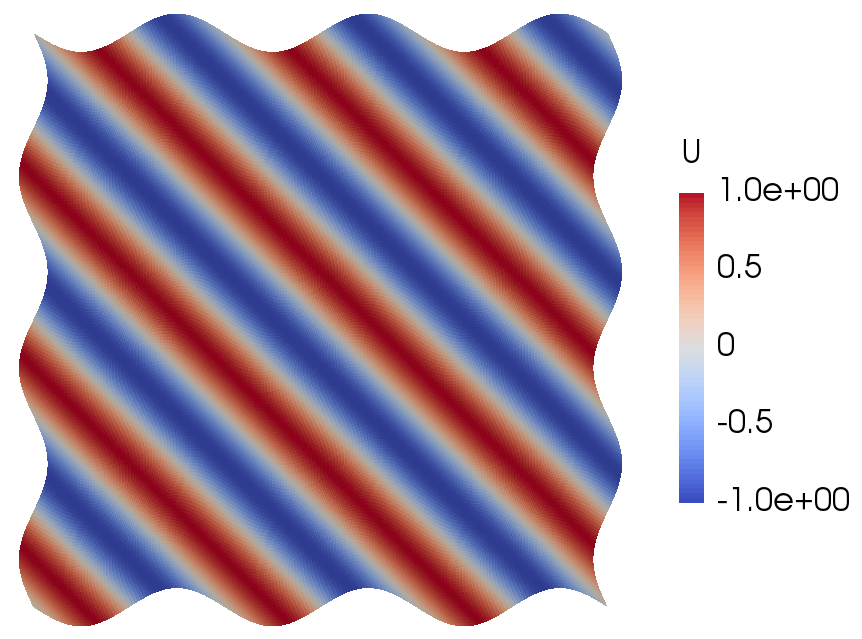
\includegraphics[scale=0.23]{plane_wave_initial.png}}{plane_wave_animation.avi}
		\end{column}
	\end{columns}	
\end{frame}
\begin{frame}{Conclusion}
	\begin{itemize}
		\item Simulated collapsing bubble using higher order fully parallel WENO based compressible multiphase flow solver developed in the lab.
		\item Solved acoustic wave equation in 2d structured and unstructured grid using WENO4-SSPRK45 scheme. 
	\end{itemize}
	Future work:
	\begin{itemize}
		\item Large scale simulation of single and multiple cavitation bubble collapse.
		\item Detailed analysis of acoustic waves emitted in the collapse process. 
	\end{itemize}
\end{frame}

\begin{frame}[allowframebreaks]{Bibliography}
	\frametitle{Bibliography}
	\bibliographystyle{amsplain}
	\begin{thebibliography}{99}
		\bibitem{propeller} Duttweiler M. E., Brennen C. E. Surge instability on a cavitating propeller [J]. Journal of Fluid Mechanics, 2002, 458: 133-152.
		\bibitem{animation} Supponen, Outi and Obreschkow, Danail and Kobel, Philippe and Tinguely, Marc and Dorsaz, Nicolas and Farhat, Mohamed, Shock waves from nonspherical cavitation bubbles, Physical Review Fluids 2, 093601 (2017)
		\bibitem{ADER}M. Dumbser, W. Boscheri, M. Semplice, G. Russo, Central WENO schemes for hyperbolic conservation laws on fixed and moving unstructured meshes, SIAM J. Sci. Comput. 2017 Vol.39, No. 6, pp. A2564–A2591
		\bibitem{dealii} W. Bangerth and R. Hartmann and G. Kanschat, \texttt{deal.II} -- a General Purpose Object Oriented Finite Element Library, ACM Trans. Math. Softw., Vol. 33, Issue 4 (2007), {24/1--24/27}
		\bibitem{interface} An interface capturing method for the simulation of multi-phase compressible flows
	\end{thebibliography}
\end{frame}
\begin{frame}[standout]
	Thank you!
\end{frame}
\end{document}